\documentclass{standalone}

\usepackage{tikz}
    \usetikzlibrary{arrows.meta}
    \usetikzlibrary{calc}

% \pagecolor{black}
\color{white}

\tikzset{
    pics/box frame/.style args={(#1+#2)x#3}{
        code={
            \draw rectangle (#3,#1);
            \draw rectangle (#3,-#2);
        }},
}


\begin{document}
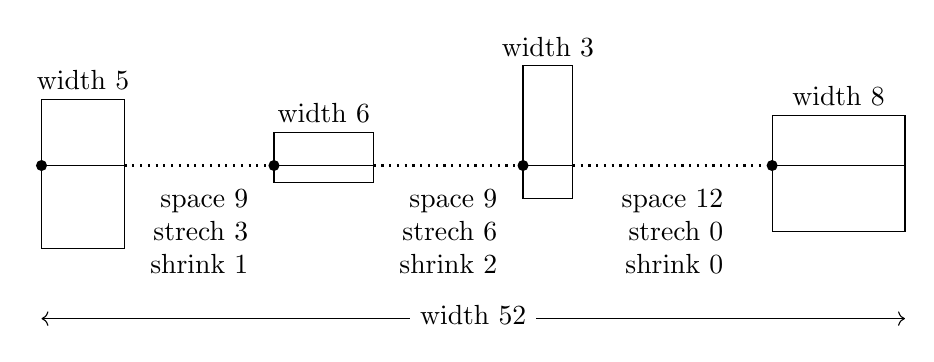
\begin{tikzpicture}[x=6pt, y=6pt]

    \def\hA{4} \def\dA{5} \def\wA{5}
    \def\hB{2} \def\dB{1} \def\wB{6}
    \def\hC{6} \def\dC{2} \def\wC{3}
    \def\hD{3} \def\dD{4} \def\wD{8}

    \def\spA{9} \def\stA{3} \def\shA{1}
    \def\spB{9} \def\stB{6} \def\shB{2}
    \def\spC{12} \def\stC{0} \def\shC{0}

    \def\gval#1#2{\csname#1#2\endcsname}

    \coordinate (bA) at (0,0);
    \coordinate (bB) at ($(bA)+(\wA+\spA,0)$);
    \coordinate (bC) at ($(bB)+(\wB+\spB,0)$)  ;
    \coordinate (bD) at ($(bC)+(\wC+\spC,0)$);

    \foreach \I in {A,B,C}{
        \draw[dotted, thick] ($(b\I)+(\gval w\I,0)$) 
            --node[below=5, align=right] {space \gval{sp}\I\\strech \gval{st}\I\\ shrink \gval{sh}\I}
            +(\gval{sp}\I, 0);
    }

    \foreach \I in {A,B,C,D}{
        \pic at (b\I) {box frame=(\gval h\I+\gval d\I)x\gval w\I};
        \fill (b\I) circle [radius=2pt];
        \node[above] at ($(b\I)+(\gval w\I/2,\gval h\I)$) {width \gval w\I};
    }

    \node (W) at ($0.5*(bD)+0.5*(\wD,0)+(0,-9)$) {width 52};
    \coordinate (X) at ($(W.base west)+(0,0.5ex)$);
    \coordinate (Y) at ($(W.base east)+(0,0.5ex)$);
    \coordinate (Z) at ($(bD)+(\wD,0)$);
    
    \draw[<-] (bA |- X) -- (X);
    \draw[->] (Y) -- (Y-|Z);

\end{tikzpicture}
\end{document}